\subsection{The Impact of Deviations of the Data from the Idealized qDF} \label{sec:results_mixedDFs}

%Motivation of the test and what we're doing
Our modelling approach assumes that each \MAP follows a quasi-isothermal distribution function, qDF. In this Section we explore what happens if this idealization does not hold. This could be, because even in the limit of perfectly measured abundances, MAPs do not follow a qDF. Or, even if they did do that, because the finite abundance errors effectively mix different MAPs.  We investigate both these issues by creating mock data sets (Fig. \ref{fig:isoSphFlexMix_mockdata}) that are drawn from two distinct qDFs of different temperature, and analyze the composite mock data set by fitting a single qDF to it. These results are illustrated in Figs. \ref{fig:isoSphFlexMixCont} and \ref{fig:isoSphFlexMixDiff}. Following the observational evidence, MAPs with cooler qDFs also have longer tracer scale lengths. In the first set of test, we choose qDFs of widely different temperatures and vary their relative fraction (dubbed ``examples 1a/b", Fig. \ref{fig:isoSphFlexMixCont}) ; in the second set of tests (``examples 2a/b", Fig. \ref{fig:isoSphFlexMixDiff}), we always mix mock data points from two different qDFs in equal proportion, but vary by how much the qDF's temperatures differ. 
\\The first set of tests mimicks a DF that has wider wings or a sharper core in velocity space than a qDF (Fig. \ref{fig:isoSphFlexMix_mockdata}). The second test could be understood by mixing neighbouring \MAPs due to too large bin sizes or abundance measurement errors.

%What we see in the plot
It is worth considering separately the impact of the DF deviations on the recovery of the potential and of the qDF parameters. 
\\We find from example 1 that the potential parameters can be better and more robustly recovered, if a mock-data \MAP is polluted by a modest fraction ($\lesssim 30\%$) of stars drawn from a cooler qDF with a longer scale length, as opposed to the same pollution of stars drawn from a hotter qDF with a shorter scale length. 
\\When considering the case of a 50/50 mix of contributions from different qDFs , there is a systematic, but only small, error in recovering the potential parameters, monotonically increasing with the qDF parameter difference (example 2); in particular for fractional differences in the qDF parameters of $\lesssim 20\%$ the systematics are insignificant even for samples sizes of 20,000, as used in the mock data. 
\\The recovery of the effective qDF parameters, in light of non qDF mock data is quite intuitive: the effective qDF temperature lies between the two temperatures from which the mixed DF of the mock data was drawn; in all cases the scale length of the velocity dispersion fall-off, $h_{\sigma R}$ and $h_{\sigma , z}$, is shorter, because the stars drawn form the hotter qDF dominate at small radii, while stars form the cooler qDF (with its longer tracer scae length) dominate at large radii. The recovered tracer scale lengths, $h_R$ vary smoothly between the input values of the two qDFs that enetered the mix of mock data, with again the impact of contamination by a hotter qDF (with its shorter scale length in this case) being more important. 

%Physical interpretation (written by Wilma alone)
%We interpret the results in example 1 as recovering the potential from a DF, whose velocity dispersion has a steeper core and more stars at larger radii than expected (reddish data sets in Fig. \ref{fig:isoSphFlexMix_mockdata}), or a DF that has broader velocity dispersion wings and more stars at small radii than predicted by the qDF (bluish data sets). We find that the former would give more reliable results for the potential parameter recovery. At the same time, if we assume that the distribution of stars from one \MAP is caused by radial migration away from the initial location of star formation, it is more likely that the qDF overestimates the true number of stars at smaller radii. [TO DO: Is this actually a sensible argument???] This could be remedied by focusing the analysis especially on hotter \MAPs with shorter scale length, for which pollution by colder stars is also much less a problem.
%\\Example 2 could be understood as a model scenario for decreasing bin sizes in the metallicity-$\alpha$ plane when sorting stars in different \MAPs, assuming that there is a smooth variation of qDF within the metallicity-$\alpha$ plane and each \MAP indeed follows a qDF. We find that, in the case of 20,000 stars in each bin, differences of $20\%$ in the qDF parameters of two neighbouring bins can still give quite good constraints on the potential parameters. We compare this with the relative difference in the qDF parameters in the bins in fig. 6 of \cite{bov13}, which have sizes of $[Fe/H] = 0.1$ dex and $\Delta [\alpha/Fe] = 0.05$ dex. It seems that these bin sizes are large enough to make sure that $\sigma_{R,0}$ and $\sigma_{z,0}$ of neighbouring \MAPs do not differ more than $20\%$. As fig. \ref{fig:isoSphFlexMixCont} and \ref{fig:isoSphFlexMixDiff} suggests especially the tracer scale length $h_R$ needs to be recovered to get the potential right. For this parameter however the bin sizes in fig. 6 of \cite{bov13} might not yet be small enough to ensure no more than $20\%$ of difference in neighbouring $h_R$, especially in the low-$\alpha$ ($[\alpha/Fe] \lesssim 0.2$), intermediate-metallicity ($[Fe/H] \sim -0.5$) \MAPs - provided of course, that each bin contains 20,000 stars. In case there are less than 20,000 stars in each bin the constraints are less tight and due to Poisson noise one could also allow larger differences in neighbouring \MAPs while still getting reliable results.


\paragraph{Further notes:} [TO DO] Mention, that vcirc is more tightly constraint with cool MAP. 

%====================================================================

%FIGURE: isoSphFlexMix_mockdata_residuals

\begin{figure*}
\plotone{figs/isoSphFlexMix_mockdata_residuals.eps}
\caption{Distribution of mock data, created by mixing stars drawn from two different qDFs (solid lines), and the distribution predicted by the best fit of a single qDF and potential to the data (dashed lines). The model parameters to create the data are given in Table \ref{tab:tests} as test \textcircled{7}, and the qDF parameters referenced in the figure's legend in Table \ref{tbl:referenceMAPs}. \emph{Example 1:} Distribution of mock data drawn from a superposition of two very different (but fixed) qDFs at varying mixing rates. \emph{Example 2:} Mock data distribution of two \MAPs that were mixed at a fixed rate of 50\%/50\%, but the difference of the qDF parameters of one \MAP was varied with respect to the qDF parameters of the other \MAP by $X\%$ (see Table \ref{tbl:referenceMAPs}). The data sets are color coded in the same way as the corresponding analyses in Fig.  \ref{fig:isoSphFlexMixCont} and \ref{fig:isoSphFlexMixDiff}. This figure demonstrates how mixing two qDFs can be used as a test case for changing the shape of the DF to not follow a pure qDF anymore, e.g. by adding wings or slightly changing the radial density profile. A second set of mock data was drawn from a single qDF and the best fit parameters found in Fig.  \ref{fig:isoSphFlexMixCont} and \ref{fig:isoSphFlexMixDiff} and overplotted as dashed lines. Especially for the most extreme deviations between mock data and best fit distribution it becomes obvious that a single qDF is a bad assumption for the stars' "true" DF. [TO DO: make larger distance between the top and bottom panels.] [TO DO: Write "mixture of 2 qDFs" in legend]}
\label{fig:isoSphFlexMix_mockdata_residuals}
\end{figure*}


%FIGURE: isoSphFlexMixCont

\begin{figure*}
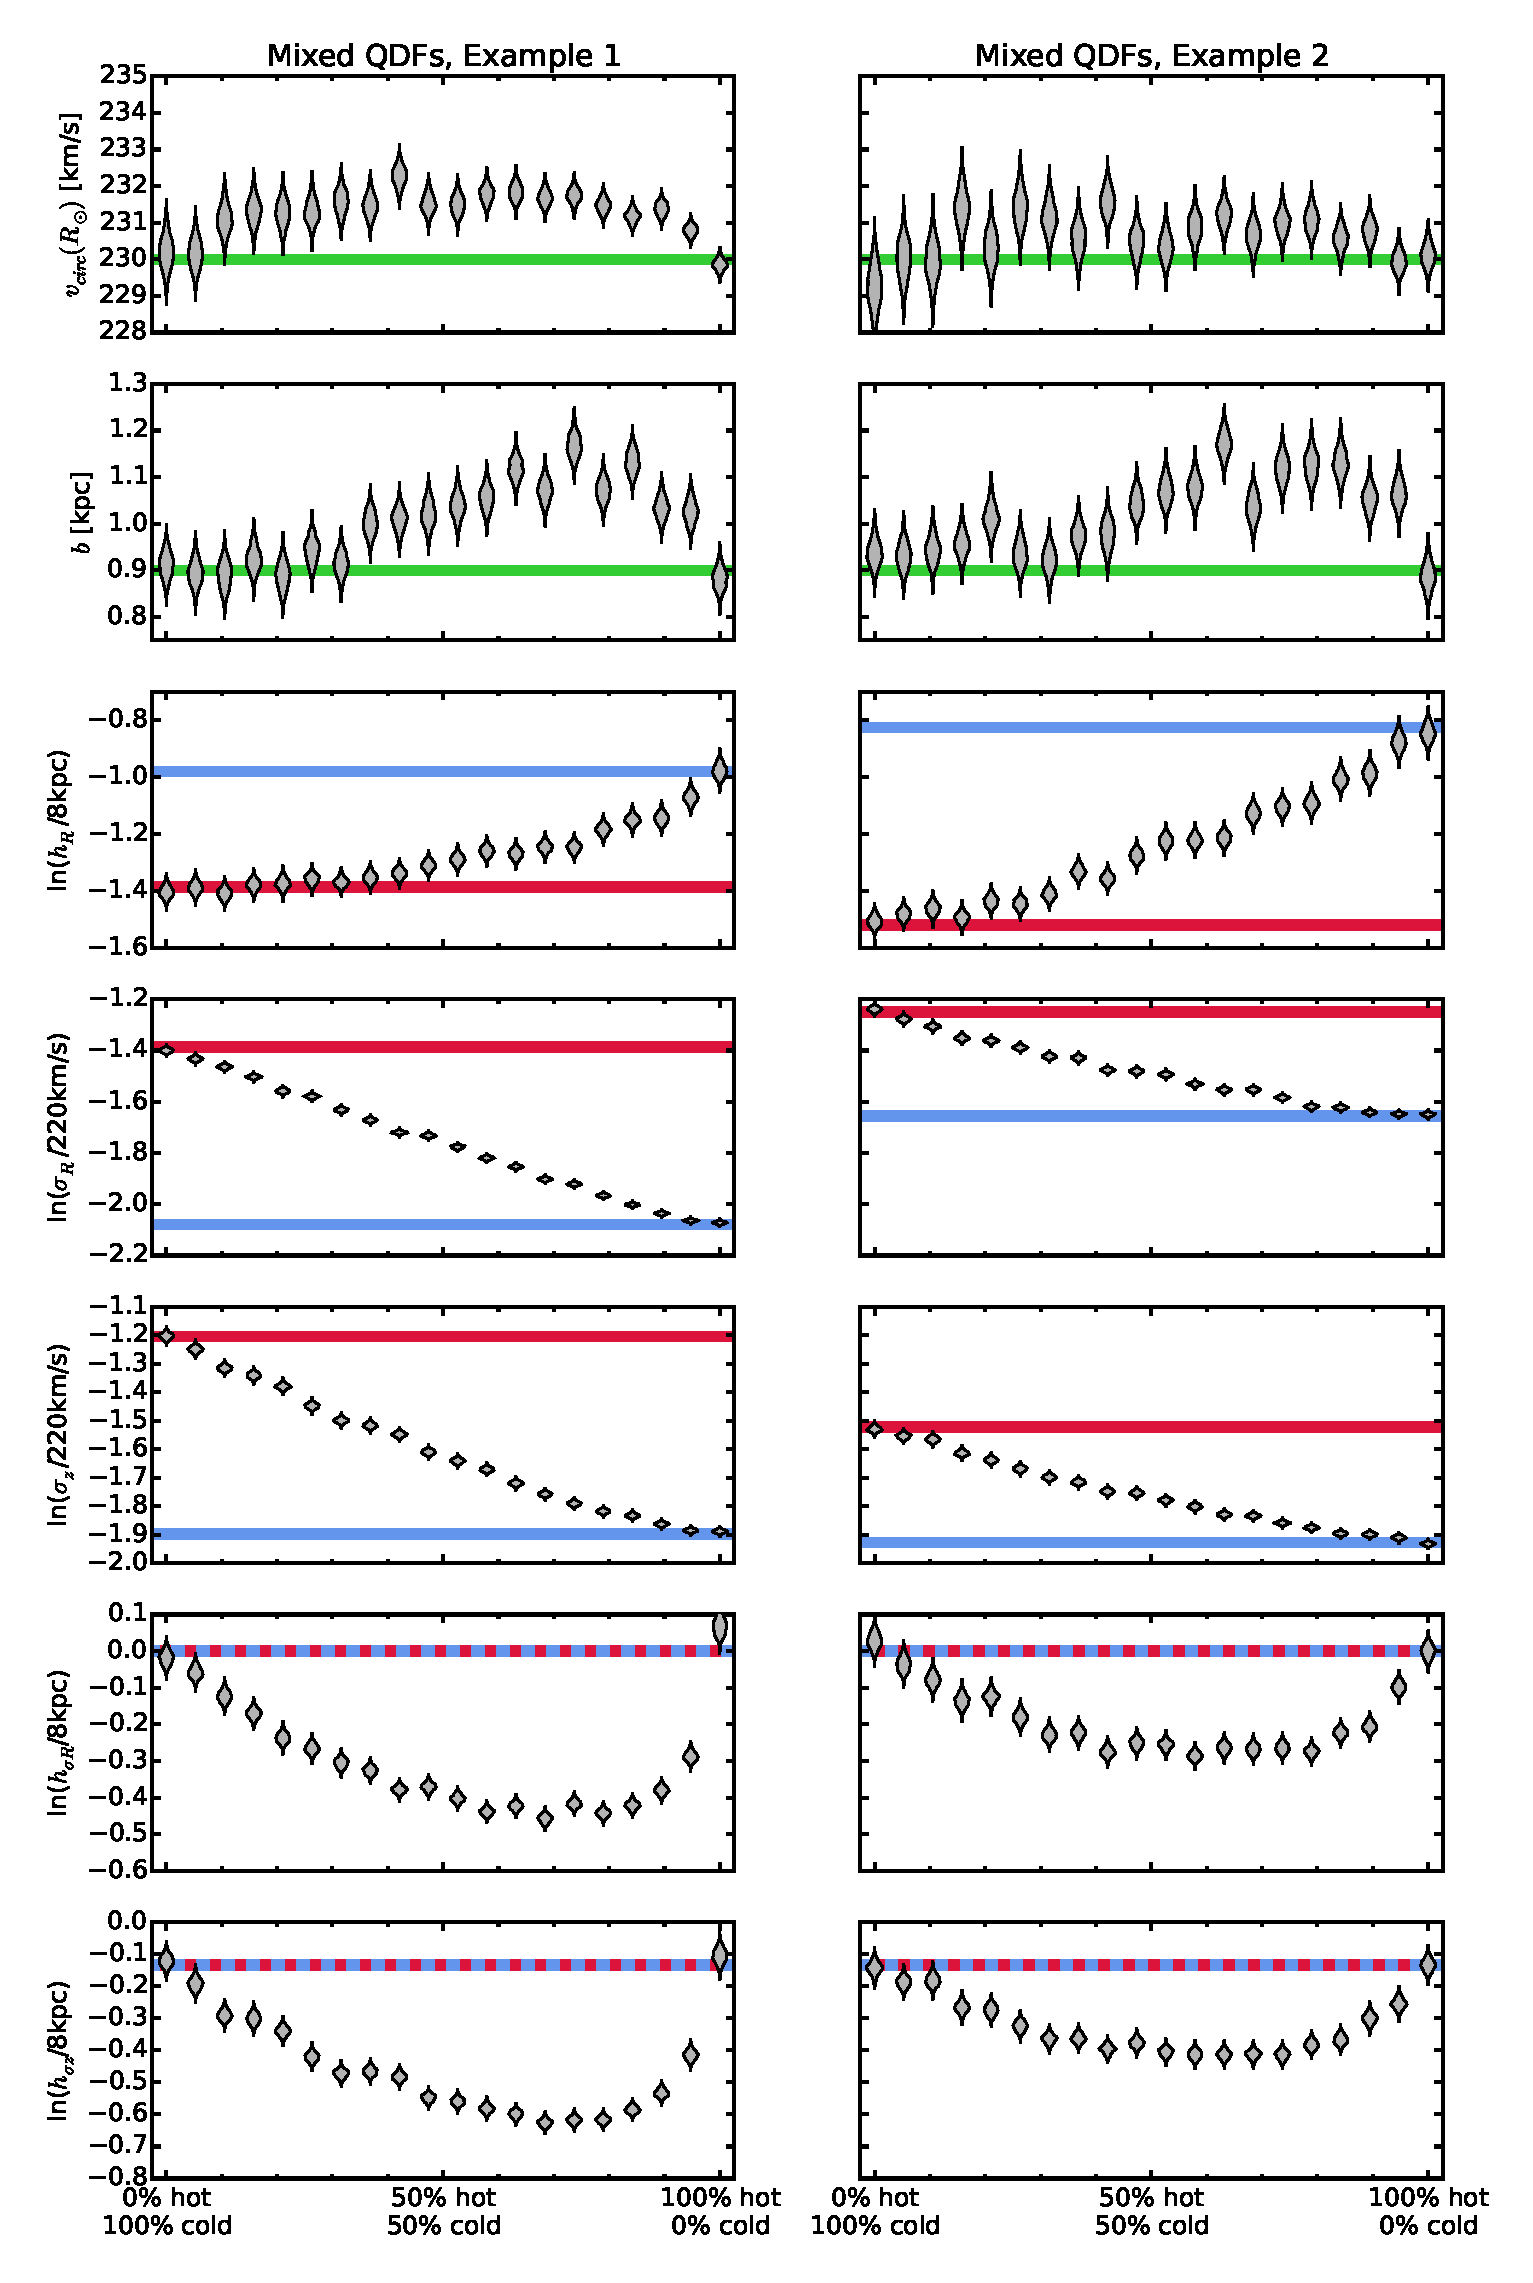
\includegraphics[width=0.8\textwidth]{figs/isoSphFlexMixCont_violins.eps}
\caption{[TO DO: Update caption.] The dependence of the parameter recovery on degree of pollution and 'hotness' of the stellar population. To model the pollution of a hot stellar population by stars coming from a cool population and vice versa, we mix varying amounts of stars from two very different populations, as indicated on the $x$-axis. The composite mock data set is then fit with one single qDF. The violines represent the marginalized likelihoods found from the MCMC analysis. The mock data sets are shown in fig. \ref{fig:isoSphFlexMix_mockdata}, in the same colors as the violins here. All mock data sets come from the same potential ("Iso-Pot") and selection function (sphere with $r_\text{max} = 2$ kpc). The true potential parameters are indicated by green dotted lines. Example 1 (Example 2) in the left (right) panels mixes the "hot" ("cool") \MAP with the "cooler" ("hotter") \MAP in table \ref{tbl:referenceMAPs}. True parameters of the hotter (colder) of the two populations are shown as red (blue) dotted lines. We find, that a hot population is much less affected by pollution with stars from a cooler population than vice versa.  [TO DO: This was done using the current qDF to set the fitting range. Nvelocity=24 and Nsigma=5 is high enough (though not perfect). Maybe redo with fiducial qDF to be consistent with MixDiff test. ???] [TO DO: Rename example 1 \& 2 to example 1a/1b and example 3 \& 4 to example 2a/2b] [TO DO: Legend]}
\label{fig:isoSphFlexMixCont}
\end{figure*}

%FIGURE: isoSphFlexMixDiff

\begin{figure*}
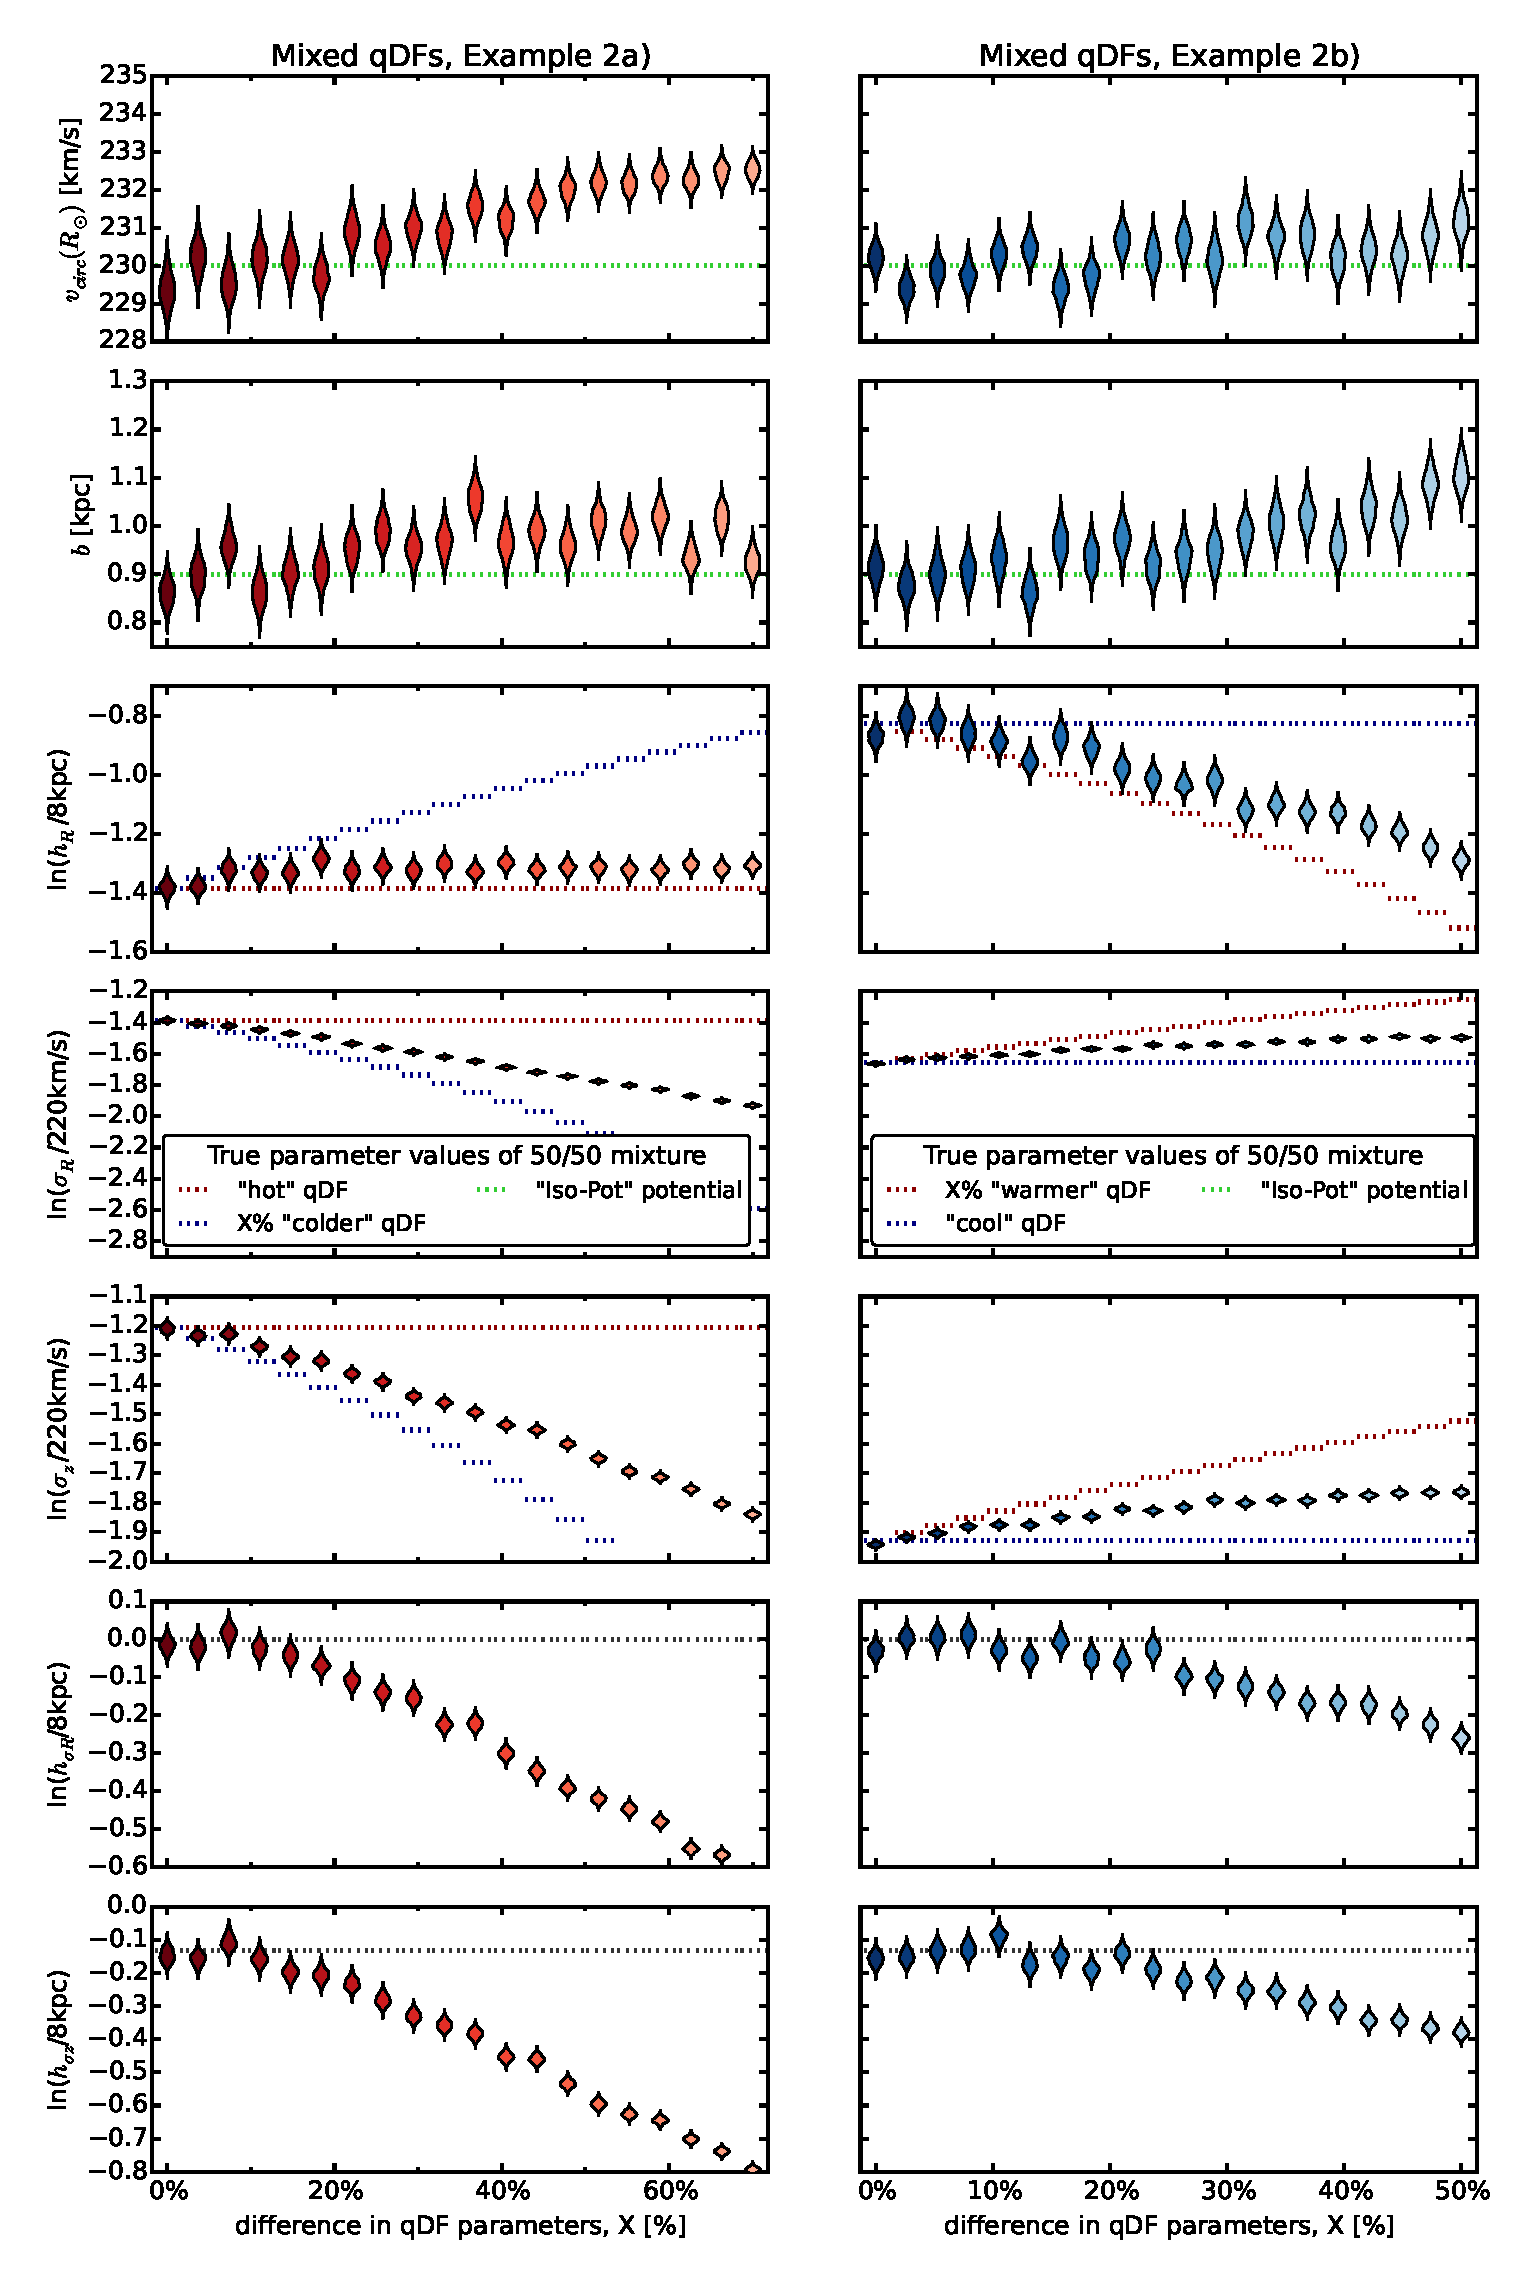
\includegraphics[width=0.8\textwidth]{figs/isoSphFlexMixDiff_violins.eps}
\caption{[TO DO: Update caption.] The dependence of the parameter recovery on the difference in qDF parameters of the 50\%/50\% mixture of two stellar populations and their 'hotness'. Each mock data set in Example 3 (Example 4) consists of 20,000 stars, half of them drawn from the "hot" ("cool") qDF in table \ref{tbl:referenceMAPs}, and the other half drawn from a "colder" ("warmer") population that has $X\%$ smaller (larger) $\sigma_R$ and $\sigma_z$ and $X\%$ larger (smaller) $h_R$. The difference $X$ in these qDF parameters is indicated on the $x$-axis, and the true parameters of the two qDFs are indicated by the dotted red and blue lines. Each composite mock data set is fitted by a single qDF and the marginalized MCMC likelihoods for the best fit parameters are shown as violines in the third (fourth) column of panels. The mock data was created within the same potential ("Iso-Pot") and selection function (sphere with $r_\text{max} = 2$ kpc). The true potential parameters are indicated by green dotted lines. The data sets are shown in figure \ref{fig:isoSphFlexMix_mockdata}, where the histograms have the same colors as the corresponding best fit violines here. By mixing \MAPs with varying difference in their qDF parameters, we model the effect of bin size in the [Fe/H]-[$\alpha$/Fe] plane when sorting stars into different \MAPs: The smaller the bin size, the smaller the difference in qDF parameters of stars in the same bin. We find that the bin sizes should be chosen such that the difference in qDF parameters between neighbouring \MAPs is less than 20\%.
[TO DO: Maybe different/same x-axis???] [TO DO: This was done using the current qDF to set the fitting range. Nvelocity=24 and Nsigma=5 is not high enough for the largest differences, i.e. grid search and MCMC converge to different values. Redo with fiducial qDF.] [TO DO: Add in plot a label, that it is a 50\%/50\% mix of a hot and a cold population.??] [TO DO: Rename example 1 \& 2 to example 1a/1b and example 3 \& 4 to example 2a/2b] [TO DO: Write in plot, that there is a 50/50 mix of cool and hot] [TO DO: Adapt colors to fit the residuals plot] [TO DO: Write free parameter $X$ on x-axis.] [TO DO: Legend])} 
\label{fig:isoSphFlexMixDiff}
\end{figure*}

%====================================================================
